\input ../SlidePreamble
\input ../preamble

\begin{document}

{\Huge

  \centerline{\bf TTIC 31230, Fundamentals of Deep Learning}
  \bigskip
  \centerline{David McAllester, April 2019}

\vfill
  \centerline{\bf The Quest for Artificial General Intelligence (AGI)}
  
  \vfill

\slide{Review: Chomsky vs. Kolmogorov}

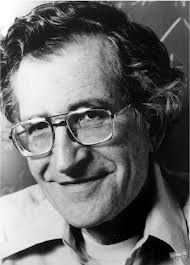
\includegraphics[width=1.0 in]{../images/Chomsky} \begin{minipage}[b]{8in} Noam Chomsky: 
  By the no free lunch theorem {\bf natural language grammar is unlearnable without an innate linguistic capacity}. In any domain a strong prior (a learning bias)
  is required. \end{minipage}

\vfill
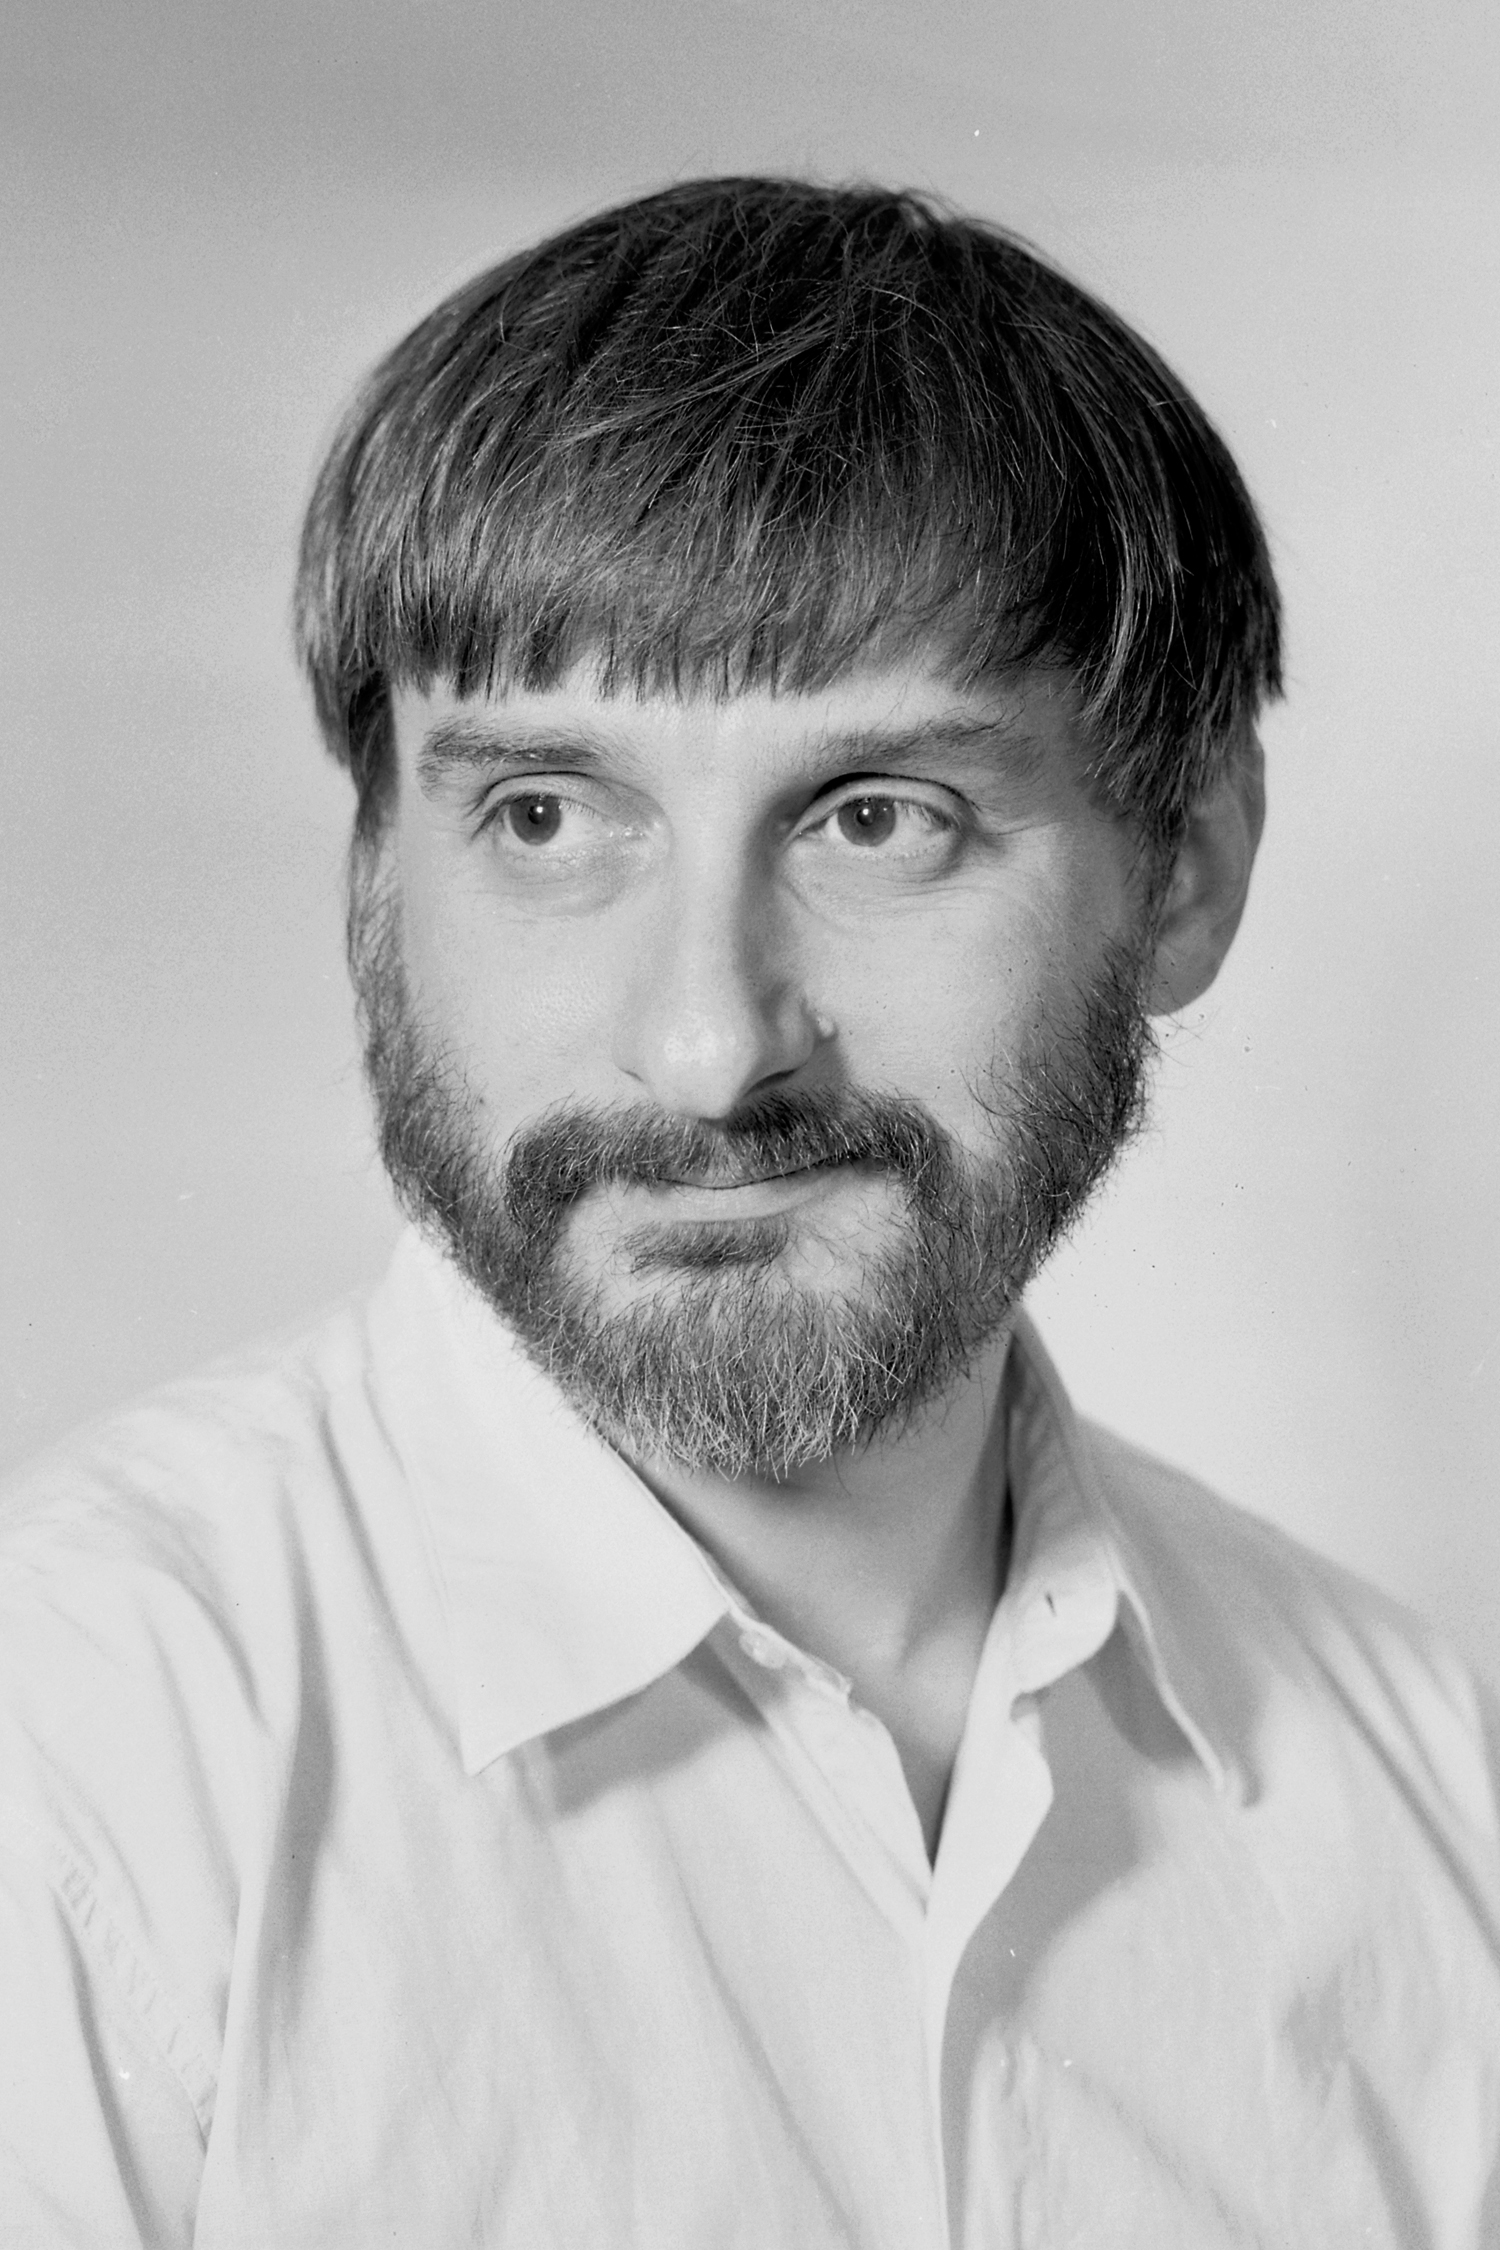
\includegraphics[height=1.0 in]{../images/Levin}
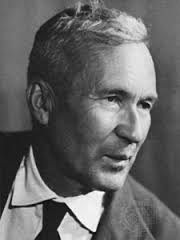
\includegraphics[height=1.0 in]{../images/Kolmogorov}
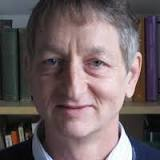
\includegraphics[height=1.0 in]{../images/Hinton}
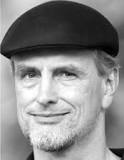
\includegraphics[height=1.0 in]{../images/Schmidhuber}

\begin{minipage}[b]{7in}
  Leonid Levin, Andrey Kolmogorov, Geoff Hinton and J\"{u}rgen Schmidhuber: {\bf Universal learning algorithms exist.
  No domain-specific innate knowledge is required.}
\end{minipage}

\slide{Review: The Free Lunch Theorem}

Consider any fixed language for naming functions. For example C++. (or English?)

\vfill
Let $|f|$ be the number of bits it takes to name function $f$ in that langauge.

\vfill
For $z \sim \pop$, let ${\cal L}(f,z) \in [0,L_{\mathrm{max}}]$ be a bounded loss function.

\vfill
{\bf Free Lunch Theorem:} With probability at least $1-\delta$ over the draw of training data $z_1,\;\ldots,\;z_N$ from $\pop$,
the following holds {\em simultaneously} for all nameable functions $f$
$${\cal L}(f) \leq\frac{10}{9}\parens{\widehat{\cal L}(f) + \frac{5L_{\mathrm{max}}}{N}\parens{(\ln 2)|f| + \ln\frac{1}{\delta}}}$$

\slide{Function Representations}

Consider continuous functions $f: [0,1]^N \rightarrow \reals$

\vfill
\vfill
\centerline{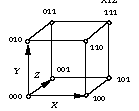
\includegraphics[width = 2in]{../images/n-cube} 
\begin{minipage}[b]{2.0in}
  $\stackrel{f}{\rightarrow} \;\;\;\reals$ \newline
  \vspace{2ex}
\end{minipage}}

\vfill
Given the corner values, the interior can be filled.

$$f(x_1,\ldots,x_N) = E_{y_1,\ldots,y_N \sim \mathrm{Round}(x_1,\ldots,x_N)}\;f(y_1,\ldots,y_n)$$

\vfill
Hence each of the $2^N$ corners has an independent value.

\slide{The Kolmogorov-Arnold representation theorem (1956)}

For continuous $f: [0,1]^N \rightarrow \reals$ there exists continuous
``activation functions'' $\sigma_i: \mathbb{R} \rightarrow \mathbb{R}$ and continuous $w_{i,j} : \reals \rightarrow \reals$ such that


\vfill
$$f(x_1,\;\ldots,\;x_N)=\sum _{{i=1}}^{{2N+1}} \sigma_i \left(\sum_{j=1}^N\;w_{i,j}(x_j)\right)$$



\slide{A Simpler, Similar Theorem}

For (possibly discontinuous) $f: [0,1]^N \rightarrow \reals$ there exists (possibly discontinuous)
$\sigma, w_i: \reals \rightarrow \reals$.

\vfill
$$f(x_1,\;\ldots,\;x_N) = \sigma\left(\sum_i w_i(x_i)\right)$$

\vfill
Proof: Select $w_i$ to spread out the digits of its argument so that $\sum_i w_i(x_i)$ contains all the digits of all the $x_i$.

\slide{Cybenko's Universal Approximation Theorem (1989)}

For continuous $f: [0,1]^N \rightarrow \reals$ and $\varepsilon >0$ there exists

\vfill
\begin{eqnarray*}
  F(x) &= & \alpha^\top \sigma(Wx + \beta) \\
  \\
  & = & \sum_i \alpha_i \sigma\left(\sum_j W_{i,j} \;x_j + \beta_i\right)
\end{eqnarray*}


\vfill
such that for all $x$ in $[0,1]^N$ we have $| F( x ) - f ( x ) | < \varepsilon$.

\slide{How Many Hidden Units?}

Consider Boolean functions $f:\;\{0,1\}^N \rightarrow \{0,1\}$.

\vfill
For Boolean functions we can simply list the inputs $x^0,\;\ldots,\;x^k$ where the function is true.

\begin{eqnarray*}
  f(x) & = & \sum_k \mathbf{1}[x=x^k] \\
  \\
  \mathbf{1}[x = x^k] & \approx & \sigma\left(\sum_i W_{k,i} x_i + b_k\right)
\end{eqnarray*}

\vfill
A simpler statement is that any Boolean function can be put in disjunctive normal form.

\slide{Representing Functions as IO Tables}

Both of the previous theorems implicitly treat functions as tables of intput-output pairs.

\vfill
\centerline{
\includegraphics[height = 1in]{../images/Frown}}

\slide{Representing Functions by Circuits}

We can define functions of Boolean variables (the corners of $[0,1]^d$) with Boolean circuits or linear threshold circuits.

\vfill
We can define functions of $[0,1]^d$ with feed-forward real-valued networks (Deep models).

\slide{Circuit Complexity Theory}

Building on work of Ajtai, Sipser and others, Hastad proved (1987) that any bounded-depth Boolean circuit computing the parity function must have exponential size. 

\vfill
Matus Telgarsky recently gave some formal conditions under which shallow networks provably require exponentially more parameters than deeper networks (COLT 2016).

\slide{Representing Functions with Programs}

Neural Turing Machines
Alex Graves, Greg Wayne, Ivo Danihelka, 2014

\vfill
(Actually a differentiable Von Neumann architecture)

\vfill
\centerline{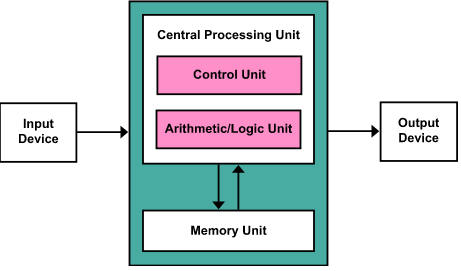
\includegraphics[height = 3in]{../images/VNA}}

\vfill
The machine undergoes discrete time state transitions defined a differentiable feed-forward circuit.

\slideplain{Discrete Time Differentiable State Transitions}

The state is defined by a state vector --- perhaps analogous to the hidden state of a gated RNN --- plus read address registers
and write address registers and a memory consisting of a (larger) set of data registers.

\vfill
Reading and writing to the data registers involves attentions over the memory defined by the address registers.


\slide{An Execution Cycle}

\vfill
The CPU receives an external input.

\vfill
The first step is to recompute the attention vectors in the read address registers.

\vfill
The CPU computes a ``key'' $k^h$ for each head $h$ and an attention $\alpha_j^h$

\begin{eqnarray*}
  \alpha^h_j & = & \softmax_j\;k^h \cdot M[j] \\
  \\
  r^h & = & \sum_j \alpha_j^h M[j]
\end{eqnarray*}

\slide{Reading from Memory}

After reading from memory the machine computes a key and attention for each write head.

\vfill
Each write operation involves ``forget'' and ``input'' operation analogous to an LSTM.

\vfill
Finally the next hidden state is computed and emitted.

\slidetwo{Compositional Attention Networks for Machine Reasoning}{Hudson and Manning, ICLR 2018}

\centerline{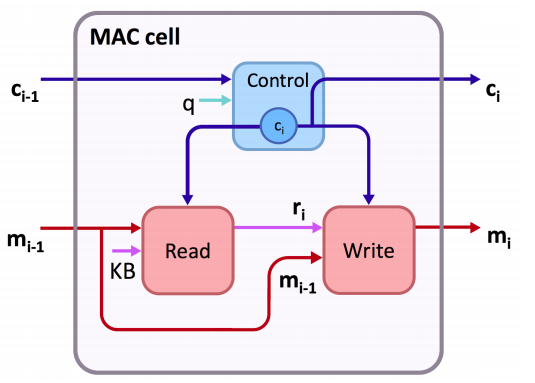
\includegraphics[height = 2.0in]{../images/MACcell}}

The MAC cell is similar to a gated RNN cell used as the decoder in translation.

\vfill
It is also similar to a Neural Turing Machine.

\vfill
It was applied to image-based question answering and uses attention over the image and the question during multi-step ``decoding''.

\slide{The Turing Tarpit}

The choice of programming language does not matter.

\vfill
For any two Turing universal languages $L_1$ and $L_2$ there exists a compiler $C: L_1 \rightarrow L_2$ such that

$$|C(h)| \leq |h| + |C|$$

\slidetwo{Deep Learning for NLP}
{vs. NLP for Deep Learning}

Progress in an application area, such as vision, can lead to progress in deep learning, such as ResNet.

\vfill
What can we learn about learning and representation (AGI) by working in NLP?

\vfill
Will the Transformer (motivated by phrase structure) replace ResNet?

\slide{The Procedural vs. Declarative Debate}

Any Discussion today of the ``knowledge representation problem'' is likely to entail a debate between proponents of {\bf declarative} and {\bf procedural} representations of knowledge.

\vfill
\rightline{Terry Winograd, 1974}

\vfill
Programming Languages (Procedural)

\vfill
vs. Natural Language (Declarative)

\slide{Natural Language Semantics}

Thousands of civilians have fled advances by Syrian government forces in eastern Ghouta as ...

\slide{Stanford Parse Tree}
\begin{verbatim}
(NP (NP (NNS Thousands))
    (PP (IN of) (NP (NNS civilians))))
(VP (VBP have)
    (VP (VBN fled)
        (NP (NNS advances))
        (PP (IN by) (NP (NP (JJ Syrian)
                            (NN government)
                            (NNS forces))
                        (PP (IN in) (NP (JJ eastern)
                                        (NNP Ghouta))))))))
\end{verbatim}

\slideplain{Stanford Dependencies}

\begin{verbatim}
root(ROOT-0, fled-5)
  aux(fled-5, have-4)
  nsubj(fled-5, Thousands-1)
    nmod(Thousands-1, civilians-3)
      case(civilians-3, of-2)
  dobj(fled-5, advances-6)
  nmod(fled-5, forces-10)
    case(forces-10, by-7)
    amod(forces-10, Syrian-8)
    compound(forces-10, government-9)
    nmod(forces-10, Ghouta-13)
      case(Ghouta-13, in-11)
      amod(Ghouta-13, eastern-12)
\end{verbatim}

\slideplain{Just Parantheses}

\begin{verbatim}
(Thousands of civilians)
(have fled)
(advances (by (Syrian government forces))
          (in eastern Ghouta))
\end{verbatim}


\slide{Natural Language: Parsing}

A Fast and Accurate Dependency Parser using Neural Networks,
Danqi Chen and Christopher Manning, 2014.

\vfill
$$\begin{array}{lllll}
  \vdots \\
  s_3 \\
    s_2 \\
    {\color{red} s_1} \\
    * & {\color{red} b_1} & b_2 & b_3 & \ldots
  \end{array}
  \;\;\;\;
  \stackrel{\mbox{push}}{\Rightarrow}
  \;\;\;
  \begin{array}{lllll}
    \vdots \\
    s_2 \\
    {\color{red} s_1} \\
    {\color{red} b_1} \\
    * & b_2 & b_3 & b_4 & \ldots
  \end{array}$$

\slide{Arc Transitions}

$$\begin{array}{llll}
    \begin{array}{lllll}
      \vdots \\
      s_3 \\
    {\color{red} s_2} \\
    {\color{red} s_1} \\
    * & b_1 & b_2 & b_3 & \ldots
  \end{array}
  &
  \stackrel{\mbox{LeftArc}}{\Rightarrow}
  &
  \begin{array}{lllll}
    \vdots \\
    s_4 \\
    s_3 \\
    {\color{red} s_1} \\
    * & b_1 & b_2 & b_3 & \ldots
  \end{array}
  &
  \mbox{Emits} \;s_1 \stackrel{{\color{red} L}}{\rightarrow} s_2 \\
  \\
  \\
    \begin{array}{lllll}
      \vdots \\
      s_3 \\
    {\color{red} s_2} \\
    {\color{red} s_1} \\
    * & b_1 & b_2 & b_3 & \ldots
  \end{array}
  &
  \stackrel{\mbox{LeftArc}}{\Rightarrow}
  &
  \begin{array}{lllll}
    \vdots \\
    s_4 \\
    s_3 \\
    {\color{red} s_2} \\
    * & b_1 & b_2 & b_3 & \ldots
  \end{array}
  &
  \mbox{Emits} \;s_2 \stackrel{{\color{red} R}}{\rightarrow} s_1 \\
\end{array}
$$

\slide{Dependency Parsing Machine Configurations}

A machine configuration

$$c = (s,b,A)$$

\begin{eqnarray*}
  s & \sim & \mbox{stack} \\
  \\
  b & \sim & \mbox{buffer} \\
  \\
  A & \sim & \mbox{Dependency Arcs}
\end{eqnarray*}

\slide{Training}

Construct a database of machine configurations labeled with actions.

\vfill
Train an MLP with one hidden layer to a softmax over actions and train on cross entropy.

\vfill
The input to the MLP is a concatenation of 18 word vectors defined in terms of the configuration

\vfill
plus 18 corresponding part of speech vectors

\vfill
and 12 parent edge label vectors.

\slideplain{Reference (Entity Linking)}

{\color{blue} Thousands of civilians have fled advances by Syrian government forces in eastern Ghouta as}
Damascus makes rapid gains against the last major rebel enclave near the capital.

\vfill
Damascus $\Rightarrow$ Assad

\vfill
Rapid Gains $\Rightarrow$ advances-6

\vfill
the last major rebel enclave ... $\Rightarrow$ Ghouta

\vfill
the capital $\Rightarrow$ Damascus

\slide{Reference vs. Composition}

Functional programming is compositional

\vfill
$$x = f(y,z)$$

\vfill
The meaning of $x$ is computed by $f$ from the meaning of $y$ and $z$.

\vfill
But in language we typically have that $f(y,z)$ is a mention and $x$ is its referent.

\vfill
(the last (major rebel enclave) (near (the capital)))

\vfill
$$x = (\mbox{the last $Q$ $P$})$$

\slide{Logical Representations of Events}

Let $e$ range over ``events''.

\vfill
$e:\mathrm{give}(a_1,x,a_2) \Rightarrow \mathrm{had}(a_1,x,\mathrm{before}(e)) \;\wedge\; \mathrm{had}(a_2,x,\mathrm{after}(e))$

\vfill
This is related to Davidsonian semantics for natural language (1969) and the situation calculus of McCarthy and Hayes (1968).

\slide{Bottom-up Logic Programming}

Bottom-up logic programming is distinguished by its relationship to dynamic programming algorithms.

\vfill
$$\mathrm{At}(x) \Rightarrow \mathrm{Reachable}(x)$$

\vfill
$$\mathrm{Reachable}(x) \wedge \mathrm{CanGo}(x,y) \Rightarrow \mathrm{Reachable}(y)$$

\vfill
This defines a linear time algorithm for reachability.

\slide{Datalog}

A set of inference rules each of which has antecedents and conclusions that are just predicates applied to variables is called a {\bf datalog} program.

\vfill
It can be shown that datalog ``captures the complexity class $P$'' --- they can express {\bf all and only} polynomial time decidable relations
(provided the entities are assigned a total order).

\vfill
General bottom-up logic programs, including expressions (terms), are Turing complete.

$$N(x) \Rightarrow N(s(x))$$

\slide{The Curry-Howard Isomorphism}

This is an isomorphism between ``proofs'' and ``programs''.

\vfill
A proof that $x$ is reachable is a path to $x$ --- a path that can actually be taken to get there.

\vfill
Curry-Howard: $\left(\exists f:\sigma \rightarrow \tau\right) \;\;\Leftrightarrow \;\;\left(\exists \mathrm{Proof}: (\exists \sigma) \Rightarrow (\exists \tau)\right)$.

\vfill
But this is not really true --- while constructive proofs are useful, we also believe in non-constructive proofs.

\vfill
Furthermore, ``proof irrelevance'' is essential to dynamic programming.

\slide{The 17 Fundamental Particles}

\centerline{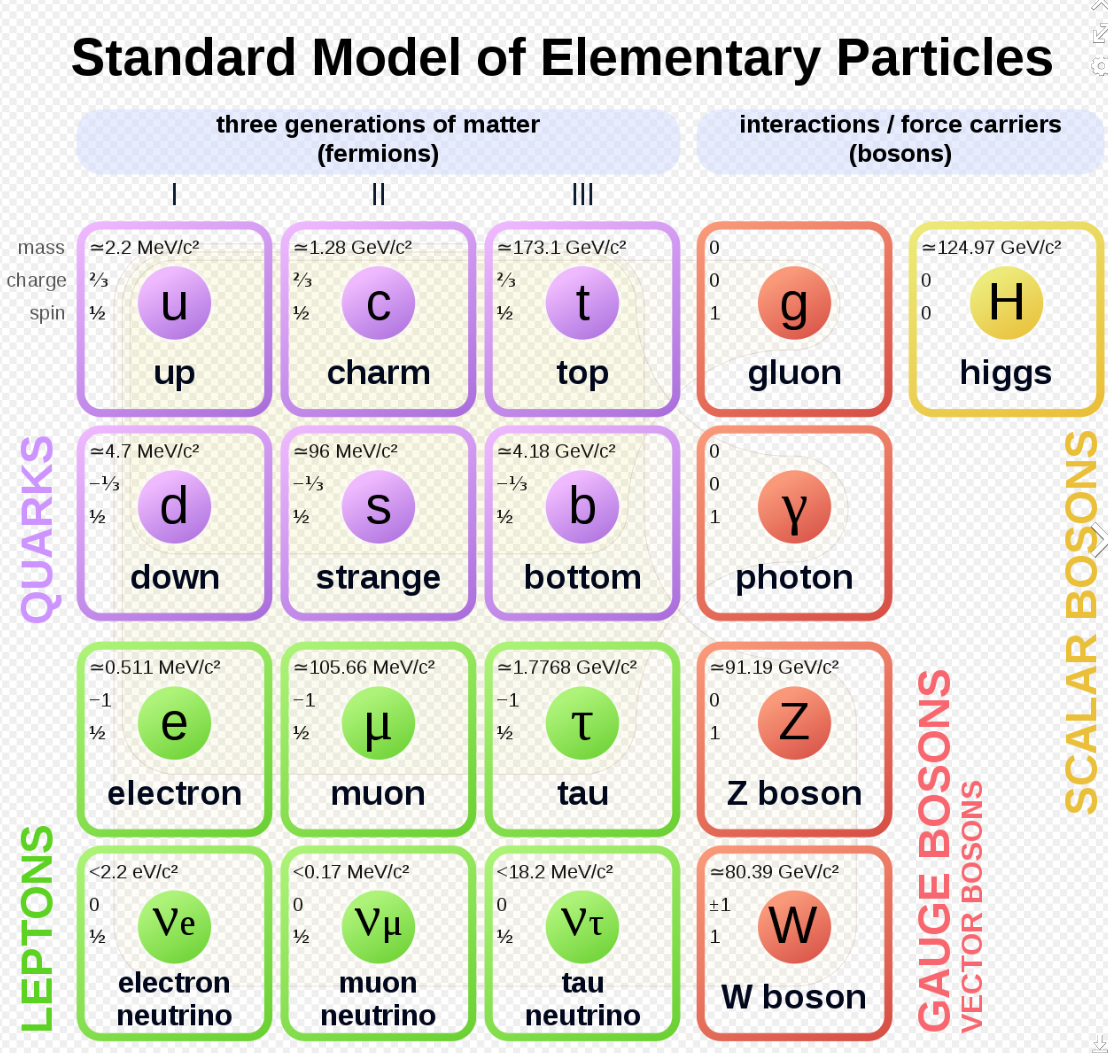
\includegraphics[height = 5.3in]{../images/StandardModel}}

\slide{17 Fundamental Constructs of Mathematics}

  $$
  \begin{array}{|l|c|c|c|c|}
  \hline
    \mbox{variables, pairs} & x & (e_1,e_2) & \pi_i(e) \\ \hline 
    \mbox{functions} & \lambda \intype{x}{\sigma}\;e[x] & f(e) & \\ \hline 
    \mbox{atoms} & ~~P(e)~~~ & ~~ e_1 \doteq e_2 ~~~~ & e_1 =_\sigma e_2 \\ \hline
    \mbox{formulas} & \neg \Phi &  \Phi_1 \vee \Phi_2 & \forall \intype{x}{\sigma}\; \Phi[x] \\ \hline
    \mbox{types}   & \Sigma_{\intype{x\;}{\;\sigma}}\;\tau[x] & \Pi_{\intype{x\;}{\;\sigma}}\;\tau[x] & S_{\intype{x\;}{\;\sigma}}\;\Phi[x]  \\ \hline
    \mbox{type constants} & \mathrm{Bool} & \mathrm{Set} & \mathrm{Type} \\ \hline
  \end{array}
  $$


\slide{The Base Case}

The base case is given by $\bool$, $\mathbf{Set}$ and $\mathbf{Type}$ with $\intype{\bool}{\mathbf{Type}}$ and $\intype{\mathbf{Set}}{\mathbf{Type}}$.


\begin{eqnarray*}
\sigma \times \tau & \doteq & \Sigma_{\intype{\alpha\;}{\;\sigma}}\;\tau \;\;\;\alpha\;\mbox{not in}\;\tau\\
\\
\\
\mathbf{Graph} & \doteq & \Sigma_{\intype{\alpha\;}{\;\mathbf{Set}}}\;(\alpha \times \alpha) \rightarrow \bool
\end{eqnarray*}

\slide{The Substitution of Isomorphics}

The isomorphism relation $u =_\sigma v$ is challenging to define in complete generality.

\vfill
But we know we want the following substitution rule.

\vfill
\centerline{
\unnamed{
\ant{\Sigma \vdash \intype{\sigma}{\type}}
\ant{\Sigma;\;\intype{x}{\tau}\vdash \intype{e[x]}\sigma}
\ant{\Sigma \vdash a=_\tau \;b}
}{
\ant{\Sigma \vdash e[a] =_\sigma e[b]}}
}

\slide{The Baldwin Effect: Learning Facilitates Adaptation}

\includegraphics[width = 1.2in]{../images/hinton}

In a 1987 paper entitled ``How Learning Can Guide Evolution'', Goeffrey Hinton and Steve Nowlan brought attention to a paper by Baldwin (1896).

\vfill
The basic idea is that by facilitating adaptation of the individual, learning facilitates evolution of the species.

\vfill
For example, longer arms are easier to evolve if arm control is learned --- arm control is then independent of arm length.  Arm control and arm structure become more modular.

\slide{The Meta-Baldwin Effect: Learning Facilitates Learning}

The Baldwin effect should apply to brain modules as well, such as vision or the motor cortex.

\vfill
By facilitating adaptation of the use of the vision module, learning facilitates the evolution of the vision module.

\vfill
By facilitating adaptation of the use of the vision module, use-learning facilitates internal-learning in the vision module.

\slidetwo{The Universality Assumption in Learning}
{and Levin's Universal Problem Solver}

Leonid Levin observed that one can construct a universal solver.  The solver takes as input a solution tester
and returns as output a solution whenever a solution exists.

  \vfill
Levin's solver is universal in the sense that it is not more than a constant factor slower than any other solver mapping testers to solutions.

\vfill
It follows that for any problem in NP, the universal solver provides a P-time algorithm whenever any such algorithm exists.


\slide{Levin's Universal Solver}
  
\vfill
We time share all programs giving time slice $2^{-|h|}$ to program $h$ where $|h|$
is the length in bits of $h$.

\vfill
The run time of the universal solver is at most
$$O(2^{-|h|}(h(n) + T(n)))$$
where $h(n)$ is the time required to run program $h$ on a problem of size $n$ and $T(n)$ is the time required to check the solution.

\vfill
Here $2^{-|h|}$ is independent of $n$ and is technically a constant.

\slide{Logic vs. Learning}

Logical theorem proving was viewed in 1960s as the path to general problem solving. (The ``general problem solver'' (GPS) Simon, Shaw and Newel, 1959).

\vfill
\includegraphics[width= 1in]{../images/schmidhuber}
Schmidhuber's answer to the failure of logic is to assume universality of a learning algorithm for learning a general problem solver. The Optimally Ordered Problem Solver (OOPS), Schmidhuber, 2002.

\slide{An Intelligence Chain Reaction?}

Let an ultraintelligent machine be defined as a machine that can far surpass all the intellectual activities of any person however clever. Since the design of machines is one of these intellectual activities, an ultraintelligent machine could design even better machines; there would then unquestionably be an ‘intelligence explosion,’ and the intelligence of humanity would be left far behind. Thus the first ultraintelligent machine is the last invention that humanity need ever make, provided that the machine is docile enough to tell us how to keep it under control.

\vfill
\rightline{I.J. Good, 1969}

\slide{END}

}
\end{document}

\ignore{
\slide{Neural Programmer Interpreter}

Neural Programmer-Interpreter, Scott Reed and Nando de Freitas, ICLR, 2016

\slide{Neural Programmer Interpreter}

We will use
\begin{eqnarray*}
i &\sim & \mbox{procedure pointer (integer)} \\
p &\sim & \mbox{procedure instruction (vector)} \\
a &\sim & \mbox{arguments (sequence of integers)} \\
e &\sim& \mbox{memory (array of vectors)} \\
h & \sim& \mbox{CPU state vector}
\end{eqnarray*}

To execute a procedure call $\mathrm{RUN}(i,a,e)$

\vfill
\begin{quotation}
$h \leftarrow 0$

$p \leftarrow  M^{\mathrm{Prog}}[i]$

\vfill
Until $f_{\mathrm{end}}(h): \;\;\;e,h \leftarrow \mathrm{DoStep}(p,a,e,h)$

\vfill
$\mathrm{return}(e)$
\end{quotation}

\slide{DoStep}

To compute $\mathrm{DoStep}(p,a,e,h)$

\vfill
\begin{quotation}
$h \leftarrow f_{\mathrm{LSTM}}(p,a,e,h)$

\vfill
$k \leftarrow f_{\mathrm{prog}}(h)$

\vfill
$i \leftarrow \argmax_i\; k^\top M^{\mathrm{Key}}[i]$

\vfill
If $i = 0:\;\;e \leftarrow f_{\mathrm{Env}}(p,f_{\mathrm{Arg}}(h),e)$

\vfill
else: $e \leftarrow \mathrm{RUN}(i,f_\mathrm{Arg}(h),e)$

\vfill
$\mathrm{return}(e,h)$
\end{quotation}


\slide{Non-Differentiable Steps}

To execute a procedure call $\mathrm{RUN}(i,a,e)$

\vfill
\begin{quotation}
$h \leftarrow 0$

$p \leftarrow  M^{\mathrm{Prog}}[i]$

\vfill
Until ${\color{red} f_{\mathrm{end}}(h)}: \;\;\;e,h \leftarrow \mathrm{DoStep}(p,a,e,h)$

\vfill
$\mathrm{return}(e)$
\end{quotation}

\slide{Non-Differentiable Steps}

To compute $\mathrm{DoStep}(p,a,e,h)$

\vfill
\begin{quotation}
$h \leftarrow f_{\mathrm{LSTM}}(p,a,e,h)$

\vfill
$k \leftarrow f_{\mathrm{prog}}(h)$

\vfill
$i \leftarrow {\color{red} \argmax_i}\; k^\top M^{\mathrm{Key}}[i]$

\vfill
If $i = 0:\;\;e \leftarrow f_{\mathrm{Env}}(p,{\color{red} f_\mathrm{Arg}(h)},e)$

\vfill
else: $e \leftarrow \mathrm{RUN}(i,{\color{red} f_\mathrm{Arg}(h)},e)$

\vfill
$\mathrm{return}(e,h)$
\end{quotation}

\slide{Training on Execution Traces}

To train they use execution traces

\vfill
$$e_t, i_t, a_t \Rightarrow  i_{t+1},a_{t+1},f_{\mathrm{end}}$$

\slide{Tail Recursion}

\vfill
Making Neural Programming Architectures
Generalize Via Recursion, Jonathon Cai, Richard Shin, Dawn Song, ICLR, 2017

\vfill
Allowing tail recursion, and explicitly labeling tail recursions in traces, significantly improves learning.

}


\slide{The CKY algorithm for context-free parsing}

Consider a grammar defined by productions of the form $S \rightarrow \mathrm{NP}\;\mathrm{VP}$ and $N \rightarrow \mathrm{Kelly}$.

\vfill
The $O(n^3)$ CKY parsing algorithm is defined by the following two rules.

$$X \rightarrow a \;\;\wedge \;\; S[i] = a \;\; \Rightarrow X[i,i+1]$$

\vfill
$$X \rightarrow YZ \;\;\wedge \;\; Y[i,j]\;\; \wedge \;\; Z[j,k] \;\;\Rightarrow X[i,k]$$
